\documentclass{clbeamer2024}

\usepackage{minted}

\usepackage{minted}
\setminted{
	breaklines=true,
	frame=single,
	bgcolor=lightgray,
	fontsize=\small,
	escapeinside=||
}

\usepackage{xcolor}
\definecolor{bg}{rgb}{0.95, 0.95, 0.92} % Couleur gris clair

\title{
	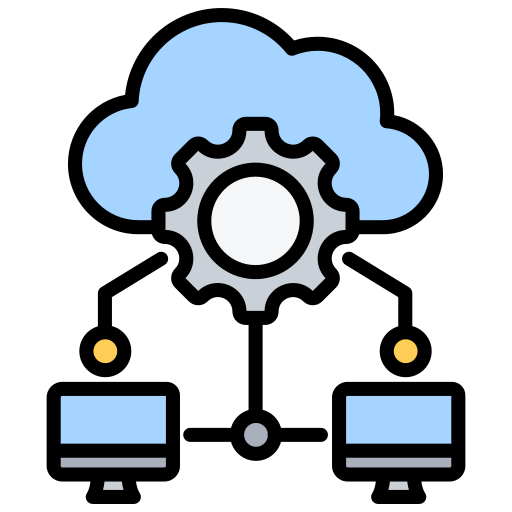
\includegraphics[width=0.8cm]{logos/tcp.png} \hfill
	TCP/UDP \hfill
	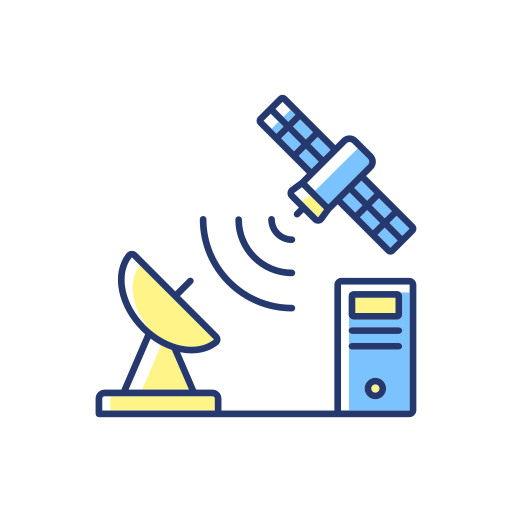
\includegraphics[width=1cm]{logos/udp.png}
}
\subtitle{Comprendre les bases des protocoles de transport}
\author{Slimani Mohamed Amine}
\institute{}
\date{\today}

\begin{document}
	\setcounter{framenumber}{-1}
	\frame{\titlepage}
	
	
	
	% Sommaire
	\begin{frame}{Sommaire}
		\tableofcontents
	\end{frame}
	

\section{Qu'est-ce que TCP ?}
\begin{frame}{Qu'est-ce que TCP ?}
	\begin{itemize}
		\item \textbf{Définition} : Protocole de transport orienté connexion, fiable et sécurisé.
		\item \textbf{Caractéristiques} :
		\begin{itemize}
			\item Livraison garantie des paquets.
			\item Contrôle de flux et de congestion.
			\item Réorganisation des paquets dans l'ordre.
		\end{itemize}
		\item \textbf{Utilisation} : Web (HTTP/HTTPS), emails (SMTP), transferts de fichiers (FTP).
	\end{itemize}
\end{frame}

\section{Qu'est-ce que UDP ?}
\begin{frame}{Qu'est-ce que UDP ?}
	\begin{itemize}
		\item \textbf{Définition} : Protocole de transport non orienté connexion, léger et rapide.
		\item \textbf{Caractéristiques} :
		\begin{itemize}
			\item Aucune garantie de livraison des paquets.
			\item Aucun contrôle de flux ou de congestion.
			\item Paquets envoyés indépendamment.
		\end{itemize}
		\item \textbf{Utilisation} : Streaming vidéo, VolP, jeux en ligne.
	\end{itemize}
\end{frame}

\section{Différences entre TCP et UDP}
\begin{frame}{Différences entre TCP et UDP}
	\begin{table}
		\begin{tabular}{|l|l|l|}
			\hline
			\textbf{Caractéristique} & \textbf{TCP} & \textbf{UDP} \\
			\hline
			Connexion & Orienté connexion & Non orienté connexion \\
			Fiabilité & Garantie de livraison & Aucune garantie \\
			Contrôle de flux & Oui & Non \\
			Vitesse & Plus lent & Plus rapide \\
			Utilisation & Données critiques & Temps réel \\
			\hline
		\end{tabular}
	\end{table}
\end{frame}

\section{Fonctionnement de TCP}
\begin{frame}{Fonctionnement de TCP}
	\begin{itemize}
		\item \textbf{Établissement de la connexion} : Poignée de main en trois étapes (SYN, SYN-ACK, ACK).
		\item \textbf{Transfert des données} : Segmentation des données en paquets numérotés.
		\item \textbf{Contrôle de flux} : Utilisation de fenêtres glissantes.
		\item \textbf{Fermeture de la connexion} : Fin de connexion en quatre étapes (FIN, ACK).
	\end{itemize}
\end{frame}


\section{Fonctionnement de UDP}
\begin{frame}{Fonctionnement de UDP}
	\begin{itemize}
		\item \textbf{Envoi des données} : Les paquets sont envoyés sans établir de connexion.
		\item \textbf{Aucun accusé de réception} : Les paquets peuvent être perdus ou arriver dans le désordre.
		\item \textbf{Léger} : Moins de surcharge par rapport à TCP.
	\end{itemize}
\end{frame}


\section{Avantages et inconvénients}
\begin{frame}{Avantages et inconvénients}
	\begin{block}{TCP}
		\textbf{Avantages} : Fiabilité, contrôle de flux, ordre des paquets. \\
		\textbf{Inconvénients} : Surcharge, plus lent.
	\end{block}
	
	\begin{block}{UDP}
		\textbf{Avantages} : Rapide, léger, idéal pour le temps réel. \\
		\textbf{Inconvénients} : Pas de fiabilité, pas de contrôle de flux.
	\end{block}
\end{frame}

\section{Exemples d'utilisation}
\begin{frame}{Exemples d'utilisation}
	\begin{itemize}
		\item \textbf{TCP} :
		\begin{itemize}
			\item Navigation web (HTTP/HTTPS).
			\item Transfert de fichiers (FTP).
			\item Envoi d'emails (SMTP).
		\end{itemize}
		\item \textbf{UDP} :
		\begin{itemize}
			\item Streaming vidéo (YouTube, Netflix).
			\item VoIP (Skype, Zoom).
			\item Jeux en ligne (Fortnite, Call of Duty).
		\end{itemize}
	\end{itemize}
\end{frame}


\section{Outils pour tester TCP/UDP}
\begin{frame}{Outils pour tester TCP/UDP}
	\begin{itemize}
		\item \textbf{netcat} : Pour envoyer des données via TCP/UDP.
		\item \textbf{Wireshark} : Pour analyser les paquets réseau.
		\item \textbf{iperf} : Pour mesurer les performances du réseau.
	\end{itemize}
\end{frame}

\section{Exemple de commandes}
\begin{frame}[fragile]{Exemple de commandes}
	\begin{exampleblock}{Commandes \texttt{netcat}}
		\begin{minted}[fontsize=\scriptsize]{bash}
# Écouter sur un port TCP
nc -l -p 1234
			
# Envoyer des données via TCP
echo "Hello TCP" | nc localhost 1234
			
# Envoyer des données via UDP
echo "Hello UDP" | nc -u localhost 1234
		\end{minted}
	\end{exampleblock}
\end{frame}


\section{Pourquoi c'est important ?}
\begin{frame}{Pourquoi c'est important ?}
	\begin{itemize}
		\item \textbf{TCP} : Essentiel pour les applications nécessitant une livraison fiable des données.
		\item \textbf{UDP} : Idéal pour les applications en temps réel où la vitesse est critique.
		\item \textbf{Comprendre les deux} : Permet de choisir le bon protocole en fonction des besoins de l'application.
	\end{itemize}
\end{frame}
	
\end{document}
